\section{Numerical Experiments}
\label{sec:experiments}

We evaluate the empirical performance of TOBYQA on the Mor\'e--Wild benchmark collection~\cite{MoreWild2009} across both stationary and drifting observation channels. The testbed comprises $65$ scalable unconstrained problems evaluated at dimensions $n \in \{6, 10, 20\}$ across $5$ independent noise realizations, for a total of $975$ problem instances per channel. Each problem is evaluated through one of the seven observation channels summarized in Table~\ref{tab:envs}. Channel amplitudes and observation noise standard deviations are scaled by the initial function magnitude $s_0 := \max(|f(\vct{x}_0)|, 1)$, with $\sigma_\varepsilon = 10^{-3} s_0$. The evaluation index advances as $t \leftarrow t + 1$ upon each function evaluation across all solvers.

\begin{table}[t]
  \centering\small
  \caption{Observation drift channels used in the benchmark experiments. Here $s_0 = \max(|f(\vct{x}_0)|, 1)$, $t$ is the sequential evaluation index, and the Lorenz trajectory is generated with standard parameters $(s, r, b) = (10, 28, 8/3)$, initial state $(1,1,1)$, and integration step $0.01$.}
  \label{tab:envs}
  \begin{tabular}{lll}
    \toprule
    Channel & Analytical Form $\phi(f(\vct{x}), t)$ & Classification \\
    \midrule
    Static        & $f(\vct{x})$                                      & Baseline ($\beta = 0$) \\
    LinearDrift   & $f(\vct{x}) + 0.01\,s_0\,t$                       & Affine drift (Theorem~\ref{thm:exact-decoupling}) \\
    PeriodicAdd   & $f(\vct{x}) + 0.05\,s_0\sin(2\pi t/50)$           & $C^2$ bounded drift (Theorem~\ref{thm:nonlinear-drift}) \\
    ChaoticDrift  & $f(\vct{x}) + 0.03\,s_0\,\mathrm{Lorenz}_x(t)$    & Chaotic dynamic drift \\
    Hetero        & $f(\vct{x}) + 0.01\,s_0\,t\,(1+\tanh\|\vct{x}-\vct{x}_0\|)$   & Spatially coupled drift \\
    MultCoupling  & $f(\vct{x})\cdot(1 + 10^{-4}t)$                   & Multiplicative drift \\
    PeriodicMult  & $f(\vct{x})\cdot(1 + 0.05\sin(2\pi t/50))$        & Multiplicative oscillatory drift \\
    \bottomrule
  \end{tabular}
\end{table}

We compare TOBYQA against representative classical and modern derivative-free solvers: Powell's interpolation solvers NEWUOA and BOBYQA~\cite{Powell2006NEWUOA,Powell2009BOBYQA} executed via the PDFO library~\cite{RagonneauZhang2024}, the noise-aware trust-region solver Py-BOBYQA~\cite{CartisRoberts2019}, the Nelder--Mead simplex search method~\cite{NelderMead1965}, and a quasi-Newton BFGS implementation using forward-difference gradient approximations ($h = 10^{-4}$). Every solver is allocated a maximum budget of $1500$ evaluations per instance. Following Mor\'e and Wild~\cite{MoreWild2009}, performance is measured on the noise-free latent objective $f$, and an instance is declared solved at accuracy tolerance $\tau \in \{10^{-1}, 10^{-3}, 10^{-5}, 10^{-7}\}$ if $\min_k f(\vct{x}_k) \le f_L + \tau(f(\vct{x}_0) - f_L)$, where $f_L$ is the smallest function value found across all solvers.

\subsection{Benchmark Comparisons}
\label{sec:bench-comparison}

\begin{table}[t]
\centering\footnotesize
\setlength{\tabcolsep}{3pt}
\caption{Solve rates (\%). Budget: 1500 evaluations per instance.}
\label{tab:solve-rates}
\begin{tabular}{lrrrrrrrrrrrr}
\toprule
Solver & \multicolumn{3}{c}{$\tau=10^{-1}$} & \multicolumn{3}{c}{$\tau=10^{-3}$} & \multicolumn{3}{c}{$\tau=10^{-5}$} & \multicolumn{3}{c}{$\tau=10^{-7}$} \\
\cmidrule(lr){2-4}\cmidrule(lr){5-7}\cmidrule(lr){8-10}\cmidrule(lr){11-13}
 & $n{=}6$ & $n{=}10$ & $n{=}20$ & $n{=}6$ & $n{=}10$ & $n{=}20$ & $n{=}6$ & $n{=}10$ & $n{=}20$ & $n{=}6$ & $n{=}10$ & $n{=}20$ \\
\midrule
\textbf{TOBYQA} & 91.4 & 88.6 & 87.3 & 70.2 & 59.9 & 41.7 & 34.4 & 32.0 & 26.2 & 28.3 & 27.7 & 24.0 \\
NEWUOA & 71.6 & 60.8 & 55.9 & 20.5 & 17.5 & 13.8 & 8.3 & 10.4 & 9.5 & 4.9 & 5.8 & 7.8 \\
Py-BOBYQA & 74.8 & 60.7 & 41.4 & 46.9 & 27.3 & 10.3 & 24.4 & 14.2 & 7.0 & 21.1 & 12.5 & 6.5 \\
Nelder--Mead & 34.2 & 19.8 & 11.7 & 8.1 & 3.6 & 3.0 & 3.2 & 2.2 & 2.8 & 1.4 & 1.0 & 1.2 \\
BFGS (FD) & 13.7 & 10.0 & 0.9 & 1.0 & 0.4 & 0.7 & 0.5 & 0.4 & 0.7 & 0.4 & 0.4 & 0.7 \\
\bottomrule
\end{tabular}
\end{table}

Table~\ref{tab:solve-rates} reports the solve rates across dimensions and convergence tolerances, while Figures~\ref{fig:data-profile} and~\ref{fig:rate-vs-tau} display the corresponding data profiles and accuracy decay curves. Across all evaluated dimensions, the performance margin of TOBYQA over the comparison solvers widens as the accuracy tolerance tightens from $\tau = 10^{-1}$ to $10^{-7}$. At loose tolerances, coarse initial steps can occasionally reduce the objective before channel drift accumulates; at high precision ($\tau \le 10^{-5}$), however, further progress requires resolving per-step objective reductions smaller than the per-step channel shift $\beta \Delta t$, where uncompensated methods stall. As reflected in the data profiles (Figure~\ref{fig:data-profile}), the baseline solvers exhaust their progress within the first $200$--$300$ evaluations, whereas TOBYQA continues to reduce the objective throughout the $1500$-evaluation budget.

\begin{figure}[t]
  \centering
  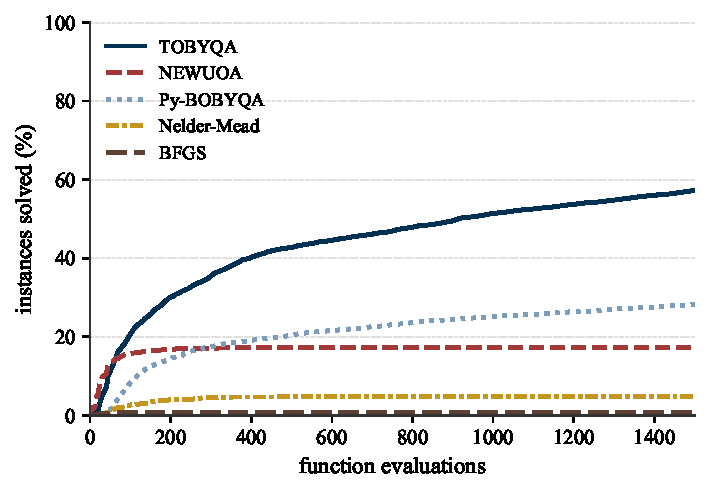
\includegraphics[width=.72\textwidth]{data_profiles_tau1e3}
  \caption{Data profiles at tolerance $\tau = 10^{-3}$: fraction of benchmark instances solved as a function of the number of function evaluations, pooled across all test problems, dimensions, and drift channels.}
  \label{fig:data-profile}
\end{figure}

\begin{figure}[t]
  \centering
  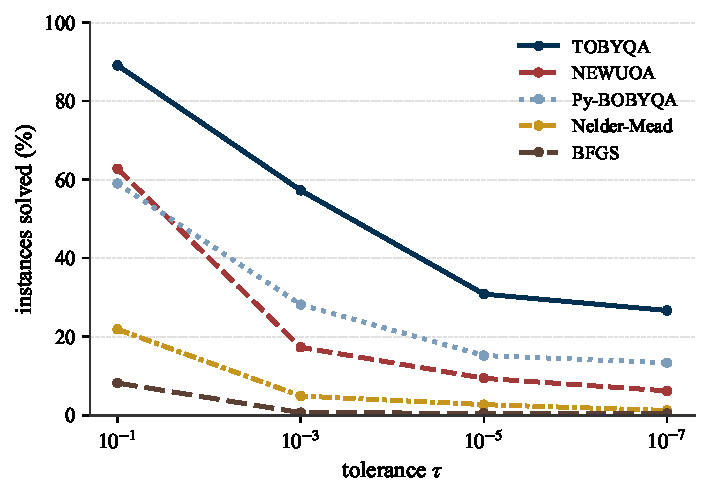
\includegraphics[width=.72\textwidth]{solve_rate_vs_tau}
  \caption{Solve rates as a function of convergence tolerance $\tau \in [10^{-7}, 10^{-1}]$, pooled across all benchmark configurations.}
  \label{fig:rate-vs-tau}
\end{figure}

The per-channel breakdown in Table~\ref{tab:env-breakdown} separates the effects of observation noise and temporal drift. On the Static channel (which still contains observation noise $\sigma_\varepsilon = 10^{-3}s_0$), unregularized interpolation solvers NEWUOA ($24.9\%$) and BOBYQA ($20.8\%$) already suffer from noise sensitivity, while TOBYQA ($57.9\%$) matches the noise-aware solver Py-BOBYQA ($59.3\%$), confirming that adding a temporal degree of freedom incurs no practical loss when drift is absent. Once additive temporal drift is introduced, however, noise robustness alone is insufficient: Py-BOBYQA drops from $59.3\%$ on Static to $4.0\%$ on LinearDrift and $3.0\%$ on Hetero, while TOBYQA achieves $64.9\%$ and $50.1\%$. Because sample points are evaluated sequentially, an unmodeled trend $\beta t$ tilts the fitted stationary quadratic surrogate along the chronological sampling path; the recovered spatial gradient absorbs this temporal trend and biases trial steps away from $-\nabla f(\vct{x}_k)$. Finite-difference BFGS fails even more severely: evaluating forward differences over consecutive steps introduces an explicit bias $(F(\vct{x}+h\vct{e}_j, t+1) - F(\vct{x}, t))/h \approx \partial f/\partial x_j + \beta/h$. With stepsize $h = 10^{-4}$ and drift rate $\beta = 10^{-2} s_0$, the drift bias $\beta/h \sim 10^2 s_0$ overwhelms the true gradient and corrupts the quasi-Newton updates.

\begin{table}[t]
\centering\footnotesize
\setlength{\tabcolsep}{3pt}
\caption{Solve rates (\%) at $\tau=10^{-3}$ broken down by drift regime, pooled over all $n$ and seeds.}
\label{tab:env-breakdown}
\begin{tabular}{lrrrrrrr}
\toprule
Solver & Chaotic & Hetero & Linear & MultCoupling & PeriodicAdd & PeriodicMult & Static \\
\midrule
\textbf{TOBYQA} & 56.0 & 50.1 & 64.9 & 56.5 & 56.2 & 59.2 & 57.9 \\
NEWUOA & 10.4 & 11.6 & 10.1 & 29.4 & 14.7 & 20.1 & 24.9 \\
Py-BOBYQA & 14.2 & 3.0 & 4.0 & 55.4 & 19.3 & 42.1 & 59.3 \\
Nelder--Mead & 1.1 & 0.0 & 0.6 & 12.3 & 3.1 & 6.3 & 10.9 \\
BFGS (FD) & 1.9 & 0.0 & 0.4 & 0.3 & 0.8 & 0.8 & 0.3 \\
\bottomrule
\end{tabular}
\end{table}

\begin{table}[t]\centering\small
\caption{Evaluation budget utilization and early termination rates across all benchmark instances.}
\label{tab:budget}
\begin{tabular}{lrrr}\toprule
Solver & Median Evals Used & \% of Budget & \% Early Termination \\\midrule
\textbf{TOBYQA} & 1500 & 100.0 & 8.5 \\
NEWUOA & 185 & 12.3 & 99.0 \\
BOBYQA & 147 & 9.8 & 99.8 \\
Py-BOBYQA & 1500 & 100.0 & 24.2 \\
Nelder--Mead & 1500 & 100.0 & 0.0 \\
BFGS (FD) & 180 & 12.0 & 99.6 \\
\bottomrule\end{tabular}\end{table}

This surrogate distortion also accounts for the evaluation counts and early termination rates in Table~\ref{tab:budget}. In classical trust-region methods (NEWUOA, BOBYQA), the trust-region radius $\Delta_k$ contracts whenever the observed reduction falls below the predicted decrease ($r_k < \eta$). Under temporal drift, candidate evaluations are penalized by the accumulated channel shift and are repeatedly rejected. As a result, the trust-region radius shrinks monotonically to its stopping threshold $\rho_{\mathrm{end}}$ without moving the center, triggering false convergence on over $99\%$ of runs at a median of only $147$--$185$ evaluations. In contrast, TOBYQA prevents premature step contraction by subtracting the estimated temporal trend from the actual reduction (Proposition~\ref{prop:ared-decomp}), while the covariance-based stopping criterion~\eqref{eq:stopping-rule} terminates only when the recovered gradient norm falls below the statistical noise floor.

\subsection{Ablation Studies}
\label{sec:ablations}

\begin{table}[t]
\centering\footnotesize
\setlength{\tabcolsep}{2.2pt}
\caption{Ablation of TOBYQA components: solve rates (\%) at $\tau=10^{-3}$ by drift regime, pooled over all $n$ and seeds.}
\label{tab:ablation}
\begin{tabular}{lrrrrrrr}
\toprule
Solver & Chaotic & Hetero & Linear & MultCoupling & PeriodicAdd & PeriodicMult & Static \\
\midrule
\textbf{TOBYQA} & 56.0 & 50.1 & 64.9 & 56.5 & 56.2 & 59.2 & 57.9 \\
\quad + interpolated $H$ & 47.4 & 55.1 & 66.4 & 61.2 & 50.6 & 63.9 & 59.5 \\
\quad -- drift comp.\ ($\gamma_k{=}0$) & 9.6 & 7.1 & 8.5 & 55.5 & 12.7 & 46.2 & 56.0 \\
\quad -- curvature kernel $A$ & 29.0 & 30.1 & 39.9 & 35.5 & 34.6 & 36.3 & 34.5 \\
\quad + Powell update & 11.9 & 18.7 & 16.9 & 14.4 & 13.4 & 14.8 & 14.5 \\
\quad frozen $\sigma$ & 39.1 & 36.3 & 38.4 & 37.6 & 38.3 & 36.1 & 36.2 \\
\bottomrule
\end{tabular}
\end{table}

Table~\ref{tab:ablation} presents an ablation study isolating the effects of drift compensation, kernel structure, curvature updates, and adaptive regularization across the seven drift channels. Suppressing drift compensation in the acceptance test ($\gamma_k = 0$ in~\eqref{eq:ared-def}) demonstrates that gradient decoupling alone is insufficient: although the spatial gradient $\vct{g}_k$ remains invariant to affine drift (Theorem~\ref{thm:exact-decoupling}), the acceptance test~\eqref{eq:noise-gate} still evaluates raw function differences. A genuine descent step ($\Delta f > 0$) is rejected whenever the channel drift over the evaluation interval exceeds the objective decrease ($\beta \Delta t > \Delta f$), which drives $\sigma_k$ upward and stalls the iterate. Consequently, while the Static solve rate is nearly unchanged ($56.0\%$ vs.\ $57.9\%$), solve rates drop to $7.1\%$--$12.7\%$ across the additive drift channels.

Replacing the curvature prior kernel $K = A + \rho^{-1} I_m$ with an isotropic ridge penalty $K = \rho^{-1} I_m$ reduces solve rates from $57.9\%$ to $34.5\%$ on Static and from $64.9\%$ to $39.9\%$ on LinearDrift. Consistent with Proposition~\ref{prop:kernel-stat}, omitting $A_{ij} = \tfrac{1}{2}(\vct{d}_i^\top \vct{d}_j)^2$ treats unmodeled quadratic residuals as spatially uncorrelated noise rather than structured curvature variation. Incorporating Powell's incremental curvature update $\|\nabla^2 Q - \nabla^2 Q_{\mathrm{prev}}\|_F^2$ degrades solve rates even further to $11.9\%$--$18.7\%$ across all channels: under temporal drift, the Hessian inherited from iteration $k-1$ reflects an outdated temporal baseline, and propagating it across iterations compounds historical drift errors. Finally, fixing the cubic regularization weight to its initial value $\sigma_k \equiv \sigma_0$ ($\gamma_1 = \gamma_2 = 1$) reduces solve rates to $36.1\%$--$39.1\%$, confirming the necessity of adapting $\sigma_k$ to local curvature and step acceptance feedback.

\begin{table}[t]
\centering\footnotesize
\setlength{\tabcolsep}{3pt}
\caption{Solve rates (\%) of the zero-Hessian default versus the interpolated Hessian, by dimension and tolerance. The first three column groups use the main budget of $1500$ evaluations; the last two use scaled budgets ($n=6$ with $450$ evaluations, $n=20$ with $5000$). Pooled over all $65$ problems, $7$ drift channels, and $5$ seeds.}
\label{tab:hessian}
\begin{tabular}{l cc cc cc cc cc}
\toprule
& \multicolumn{2}{c}{$n=6$} & \multicolumn{2}{c}{$n=10$} & \multicolumn{2}{c}{$n=20$} & \multicolumn{2}{c}{$n=6$, $b=450$} & \multicolumn{2}{c}{$n=20$, $b=5000$} \\
\cmidrule(lr){2-3}\cmidrule(lr){4-5}\cmidrule(lr){6-7}\cmidrule(lr){8-9}\cmidrule(lr){10-11}
Solver & $10^{-3}$ & $10^{-5}$ & $10^{-3}$ & $10^{-5}$ & $10^{-3}$ & $10^{-5}$ & $10^{-3}$ & $10^{-5}$ & $10^{-3}$ & $10^{-5}$ \\
\midrule
TOBYQA ($H_k \equiv 0$) & 70.2 & 34.4 & 59.9 & 32.0 & 41.7 & 26.2 & 83.3 & 64.3 & 67.1 & 45.9 \\
\quad + interpolated $H$ & 62.4 & 24.0 & 60.1 & 29.9 & 50.7 & 38.9 & 67.3 & 44.9 & 70.8 & 59.7 \\
\bottomrule
\end{tabular}
\end{table}


Table~\ref{tab:hessian} compares the default zero-Hessian Cauchy step ($H_k \equiv 0$) against a trial step computed with the interpolated Hessian $H_k = \sum_{i=1}^m \lambda_i \vct{d}_i \vct{d}_i^\top$. At $n = 6$, the zero-Hessian default achieves higher solve rates across all tolerances and budgets ($70.2\%$ vs.\ $62.4\%$ at $\tau = 10^{-3}$ under budget $1500$, and $83.3\%$ vs.\ $67.3\%$ under budget $450$). With $m = 2n+1$ samples, second-order difference quotients amplify observation noise by $O(\sigma_\varepsilon/\delta_k^2)$ over an underdetermined subspace ($n(n+1)/2 = 21$ parameters vs.\ $n-1 = 5$ curvature degrees of freedom). Forming trial steps from $H_k$ therefore inverts noise-corrupted directional curvatures, whereas the Cauchy step~\eqref{eq:closed-form-step} relies only on the fully-linear gradient $\vct{g}_k$.

At $n = 20$, the pooled solve rate in Table~\ref{tab:hessian} favors the interpolated Hessian ($50.7\%$ vs.\ $41.7\%$ at budget $1500$, and $70.8\%$ vs.\ $67.1\%$ at budget $5000$). However, the per-channel breakdown in Table~\ref{tab:ablation} shows that this gain is restricted to stationary, affine, and multiplicative channels ($59.5\%$ vs.\ $57.9\%$ on Static and $66.4\%$ vs.\ $64.9\%$ on LinearDrift), whereas on nonlinear additive drift channels the interpolated Hessian drops from $56.0\%$ to $47.4\%$ on ChaoticDrift and from $56.2\%$ to $50.6\%$ on PeriodicAdd (at $n=20$ and budget $5000$, solve rates fall to $54.5\%$ and $49.8\%$ versus $72.1\%$ and $75.7\%$ for $H_k \equiv 0$). Under nonlinear drift, the second-order temporal remainder $\vct{r}_\mu$ from Theorem~\ref{thm:nonlinear-drift} enters the dual multipliers $\vct{\lambda} = K^{-1}(\vct{F} - X_{\mathrm{aug}}\Pi\vct{F})$ directly, corrupting the eigenvalues of $H_k = \sum_{i=1}^m \lambda_i \vct{d}_i \vct{d}_i^\top$ and distorting second-order steps. For general time-varying channels with unknown drift structure, setting $H_k \equiv 0$ avoids curvature corruption from nonlinear drift while maintaining strong performance on stationary problems.

